\section{Rethinking the OPD Reward Function}
\label{sec:method}



As shown in \secref{sec:failure-modes}, post-hoc transformations of the log-ratio reward do not resolve OPD training pathologies. We therefore step back from the inherited log-ratio form and ask: \emph{what properties should a token-level OPD reward satisfy, and what functions satisfy them by construction?}

% ============================================================
\subsection{Generalizing the OPD Reward}
\label{sec:framework}
% ============================================================

The OPD log-ratio reward \(\log(\pi_T/\pi_\theta)\) is a specific mapping from teacher--student probabilities at the sampled token; we generalize it as
\begin{equation}
  r_t^{f} = f\!\left(\pi_T(o_t \mid c_t),\; \pi_\theta(o_t \mid c_t)\right),
\end{equation}
where \(f : [0,1]^2 \to \mathbb{R}\) maps a pair of teacher--student probabilities to a scalar reward. The standard OPD reward corresponds to \(f(p,q)=\log p-\log q\), which is defined on \((0,1]^2\) but diverges as \(p \to 0\) or \(q \to 0\). The post-hoc methods in \secref{subsec:standard-fixes} keep this log-ratio form fixed and only transform or normalize the rewards after they are computed. In contrast, \emph{we treat the probability-to-reward mapping \(f\) itself as the object of design}. This shifts the question from how to stabilize a pathological reward after the fact to what properties a stable OPD reward should satisfy in the first place.

% ============================================================
\subsection{Two Necessary Properties}
\label{sec:properties}
% ============================================================

We identify two necessary properties for a well-designed OPD reward.

\paragraph{P1: Boundedness.}
The reward function \(f\) should be bounded on \([0,1]^2\): there exists \(M > 0\) such that \(|f(p, q)| \leq M\) for all \(p, q \in [0,1]\). If \(f\) is unbounded, small changes in teacher or student probabilities can produce arbitrarily large reward magnitudes, directly amplifying the variance of policy-gradient updates as diagnosed in \secref{subsec:high-variance}.

\paragraph{P2: Sign Consistency.}
The sign of \(f\) should indicate which model assigns higher probability to the sampled token:
\(f(p,q)>0\) if \(p>q\), \(f(p,q)=0\) if \(p=q\), and \(f(p,q)<0\) if \(p<q\).
This ensures that token-level updates move the student toward the teacher: tokens assigned higher probability by the teacher receive positive reward, and vice versa.
If P2 is violated, updates can point in the wrong direction regardless of reward magnitude.

\paragraph{P1 and P2 explain the empirical failures.}
The failure modes in \secref{sec:failure-modes} are consistent with these two properties. \emph{Vanilla OPD} satisfies P2 but violates P1, producing the high-variance rewards diagnosed above. \emph{Z-Score} does not guarantee P1 and may violate P2 because batch centering can flip individual reward signs, explaining its poor performance in \autoref{fig:standard-fixes}. \emph{Clip} and \emph{Tanh} enforce P1 while preserving P2, and therefore improve over vanilla OPD; however, they still fail because they compress rewards only after the divergent log-ratio has been computed. Thus, P1 and P2 are minimal properties: they must hold at the probability-to-reward mapping level, before any log-ratio distortion occurs.
% ============================================================
\subsection{Deriving Rewards that Satisfy P1 and P2}
\label{sec:motivation}
% ============================================================
\begin{table*}[t]
\centering

\begin{subtable}{\linewidth}
\centering
\scriptsize
\setlength{\tabcolsep}{1.0pt}
\renewcommand{\arraystretch}{1.05}
\caption{Teacher: Qwen3-4B $\to$ Student: Qwen3-1.7B-Base}
\label{tab:main-1p7b-4b}
\begin{adjustbox}{max width=\linewidth}
\begin{tabular}{@{}ll lll@{\hskip 6pt}lll@{\hskip 6pt}lll@{\hskip 6pt}lll@{\hskip 6pt}lll@{\hskip 6pt}lll@{\hskip 6pt}lll@{\hskip 6pt}lll@{}}
\toprule
 &  & \multicolumn{3}{c}{GSM8K} & \multicolumn{3}{c}{MATH500} & \multicolumn{3}{c}{AMC23} & \multicolumn{3}{c}{AIME24} & \multicolumn{3}{c}{AIME25} & \multicolumn{3}{c}{Minerva} & \multicolumn{3}{c}{Olympiad} & \multicolumn{3}{c}{Mean} \\
Class & Param & Avg & Pass & Len & Avg & Pass & Len & Avg & Pass & Len & Avg & Pass & Len & Avg & Pass & Len & Avg & Pass & Len & Avg & Pass & Len & Avg & Pass & Len \\
\cmidrule(lr){3-5} \cmidrule(lr){6-8} \cmidrule(lr){9-11} \cmidrule(lr){12-14} \cmidrule(lr){15-17} \cmidrule(lr){18-20} \cmidrule(lr){21-23} \cmidrule(lr){24-26}
\midrule
\multirow{1}{*}{Full-vocab} & -- & \textbf{83.50} & 95.00 & 3954 & \underline{63.12} & \textbf{87.00} & 4004 & 38.44 & 65.00 & 4096 & \textbf{10.83} & \underline{23.33} & 4096 & 5.83 & \underline{20.00} & 4096 & \textbf{19.75} & \underline{32.00} & 3805 & 17.62 & 26.00 & 4096 & 34.16 & 49.76 & 4021 \\
\cmidrule(lr){1-26}
\multirow{4}{*}{Vanilla} & -- & 73.93 & \textbf{95.68} & 351 & 54.93 & 75.12 & 1156 & 31.87 & 60.00 & 2253 & 9.17 & 16.67 & 3388 & \textbf{7.08} & 13.33 & 3282 & 16.13 & 28.68 & 1038 & 23.74 & 44.15 & 2355 & 30.98 & 47.66 & 1975 \\
 & + Clip & 80.36 & 94.01 & 326 & 59.12 & 75.92 & 1162 & 31.88 & 67.50 & 2309 & 4.17 & \underline{23.33} & 3342 & 4.58 & \underline{20.00} & 3381 & 17.56 & 28.31 & 995 & 26.74 & \underline{47.41} & 2390 & 32.06 & 50.93 & 1986 \\
 & + Tanh & 82.08 & 94.62 & 331 & 59.09 & 76.04 & 1134 & 34.06 & 60.00 & 2288 & \underline{10.42} & \textbf{26.67} & 3318 & \underline{6.67} & 16.67 & 3240 & 18.06 & 30.88 & 926 & 27.17 & 46.96 & 2359 & 33.94 & 50.26 & 1942 \\
 & + Z-Score & 42.92 & 89.61 & 372 & 28.24 & 66.24 & 1235 & 15.94 & 47.50 & 2243 & 4.17 & 13.33 & 3466 & 4.17 & 13.33 & 3244 & 9.05 & 23.16 & 1062 & 14.15 & 38.81 & 2376 & 16.95 & 41.71 & 2000 \\
\cmidrule(lr){1-26}
\multirow{7}{*}{PowerOPD} & $\alpha=0.1$ & 82.46 & 94.77 & 316 & 59.66 & 76.56 & 1127 & 33.44 & 67.50 & 2184 & 8.75 & 20.00 & 3351 & \textbf{7.08} & \textbf{23.33} & 3081 & 18.11 & 29.41 & 912 & \textbf{27.76} & 47.26 & 2332 & \cellcolor{avgshade!12}33.89 & \cellcolor{passshade!49}\underline{51.26} & \cellcolor{lenshade!33}1900 \\
 & $\alpha=1$ & 82.04 & \underline{95.38} & 317 & 59.52 & \underline{76.86} & 1132 & 38.44 & 62.50 & 2176 & \underline{10.42} & \underline{23.33} & 3368 & 4.17 & 16.67 & 3136 & 18.66 & \textbf{32.35} & 935 & 27.72 & \textbf{47.56} & 2307 & \cellcolor{avgshade!36}34.42 & \cellcolor{passshade!30}50.66 & \cellcolor{lenshade!22}1910 \\
 & $\alpha=5$ & 82.68 & 95.07 & 315 & 59.96 & 76.42 & 1116 & 38.12 & 67.50 & 2136 & 8.33 & 20.00 & 3366 & 4.17 & 13.33 & 3283 & 19.07 & 31.25 & 920 & 27.28 & 47.11 & 2289 & \cellcolor{avgshade!28}34.23 & \cellcolor{passshade!12}50.10 & \cellcolor{lenshade!12}1918 \\
 & $\alpha=10$ & 83.01 & 94.69 & 315 & 59.71 & 76.10 & 1104 & 35.62 & 67.50 & 2112 & 8.33 & \textbf{26.67} & 3292 & 5.00 & 13.33 & 3188 & 18.84 & 30.15 & 909 & 27.56 & 46.67 & 2296 & \cellcolor{avgshade!18}34.01 & \cellcolor{passshade!32}50.73 & \cellcolor{lenshade!44}1888 \\
 & $\alpha=50$ & 83.11 & 94.24 & \underline{313} & 59.40 & 75.68 & 1035 & \textbf{41.88} & \textbf{75.00} & 1950 & \textbf{10.83} & \underline{23.33} & 3227 & 4.17 & 13.33 & 2876 & 17.65 & 30.15 & \underline{827} & 26.67 & 46.52 & 2160 & \cellcolor{avgshade!55}\underline{34.82} & \cellcolor{passshade!47}51.18 & \cellcolor{lenshade!54}1770 \\
 & $\alpha=100$ & 82.92 & 93.33 & \textbf{307} & 59.80 & 75.76 & \underline{1009} & 37.81 & \underline{70.00} & \underline{1857} & 8.33 & 20.00 & \underline{3011} & 6.25 & \textbf{23.33} & \underline{2732} & 17.97 & 28.31 & \textbf{823} & 27.06 & 45.78 & \underline{2042} & \cellcolor{avgshade!31}34.31 & \cellcolor{passshade!39}50.93 & \cellcolor{lenshade!64}\underline{1683} \\
 & $\alpha=500$ & \underline{83.13} & 94.31 & 316 & \textbf{64.53} & 75.72 & \textbf{997} & \underline{40.94} & \underline{70.00} & \textbf{1673} & 9.58 & \textbf{26.67} & \textbf{2776} & \underline{6.67} & \underline{20.00} & \textbf{2588} & \underline{19.58} & 31.25 & 845 & \underline{27.74} & 46.37 & \textbf{1857} & \cellcolor{avgshade!75}\textbf{36.02} & \cellcolor{passshade!75}\textbf{52.05} & \cellcolor{lenshade!75}\textbf{1579} \\
\bottomrule
\end{tabular}
\end{adjustbox}
\end{subtable}

\vspace{0.5em}

\begin{subtable}{\linewidth}
\centering
\scriptsize
\setlength{\tabcolsep}{1.0pt}
\renewcommand{\arraystretch}{1.05}
\caption{Teacher: Qwen3-8B $\to$ Student: Qwen3-1.7B-Base}
\label{tab:main-1p7b-8b}
\begin{adjustbox}{max width=\linewidth}
\begin{tabular}{@{}ll lll@{\hskip 6pt}lll@{\hskip 6pt}lll@{\hskip 6pt}lll@{\hskip 6pt}lll@{\hskip 6pt}lll@{\hskip 6pt}lll@{\hskip 6pt}lll@{}}
\toprule
 &  & \multicolumn{3}{c}{GSM8K} & \multicolumn{3}{c}{MATH500} & \multicolumn{3}{c}{AMC23} & \multicolumn{3}{c}{AIME24} & \multicolumn{3}{c}{AIME25} & \multicolumn{3}{c}{Minerva} & \multicolumn{3}{c}{Olympiad} & \multicolumn{3}{c}{Mean} \\
Class & Param & Avg & Pass & Len & Avg & Pass & Len & Avg & Pass & Len & Avg & Pass & Len & Avg & Pass & Len & Avg & Pass & Len & Avg & Pass & Len & Avg & Pass & Len \\
\cmidrule(lr){3-5} \cmidrule(lr){6-8} \cmidrule(lr){9-11} \cmidrule(lr){12-14} \cmidrule(lr){15-17} \cmidrule(lr){18-20} \cmidrule(lr){21-23} \cmidrule(lr){24-26}
\midrule
\multirow{1}{*}{Full-vocab} & -- & 80.25 & 86.50 & 4095 & \textbf{63.25} & \textbf{84.00} & 4091 & \textbf{42.19} & \underline{75.00} & 4096 & 7.08 & 16.67 & 4096 & \textbf{5.83} & \textbf{26.67} & 4096 & 17.50 & 26.00 & 4084 & 16.50 & 29.00 & 4096 & 33.23 & 49.12 & 4093 \\
\cmidrule(lr){1-26}
\multirow{4}{*}{Vanilla} & -- & 77.55 & \underline{95.07} & 323 & 57.55 & 75.88 & 1050 & 35.94 & 62.50 & 1881 & 7.08 & 20.00 & 3045 & 3.30 & 16.67 & 2957 & 17.56 & 29.78 & 892 & 23.94 & 47.11 & 2136 & 31.85 & 49.57 & 1755 \\
 & + Clip & 76.96 & 94.84 & \textbf{308} & 59.56 & 76.68 & 1062 & 38.75 & 72.50 & 2097 & 7.08 & \underline{23.33} & 3188 & 3.30 & 16.67 & 2935 & 18.43 & 30.88 & 892 & 24.65 & 46.81 & 2177 & 32.68 & 51.67 & 1808 \\
 & + Tanh & 78.02 & 94.92 & 321 & 58.82 & 76.04 & 1078 & 35.31 & 62.50 & 1996 & \underline{8.33} & \underline{23.33} & 3107 & 4.58 & \underline{20.00} & 3012 & 18.29 & \underline{31.62} & 930 & 23.96 & 47.41 & 2205 & 32.47 & 50.83 & 1807 \\
 & + Z-Score & 80.26 & \textbf{95.22} & 323 & 58.48 & 75.98 & 1084 & 36.56 & 67.50 & 2087 & 7.08 & \underline{23.33} & 3285 & 4.17 & 13.33 & 2964 & 17.42 & \textbf{31.99} & 948 & 27.02 & \underline{48.00} & 2174 & 33.00 & 50.76 & 1838 \\
\cmidrule(lr){1-26}
\multirow{7}{*}{PowerOPD} & $\alpha=0.1$ & 79.96 & 94.31 & 319 & 59.27 & 76.78 & 1087 & 36.25 & 65.00 & 2142 & \textbf{9.17} & \underline{23.33} & 3123 & 3.75 & 13.33 & 3024 & 18.43 & \textbf{31.99} & 920 & 27.09 & 47.26 & 2227 & \cellcolor{avgshade!33}33.42 & \cellcolor{passshade!12}50.29 & \cellcolor{lenshade!12}1835 \\
 & $\alpha=0.5$ & 78.22 & 94.77 & \textbf{308} & 59.29 & 76.90 & 1052 & 36.56 & 67.50 & 2087 & \underline{8.33} & \textbf{26.67} & 3195 & \underline{5.42} & \underline{20.00} & 2962 & 17.97 & 30.88 & 899 & \underline{27.78} & \underline{48.00} & 2143 & \cellcolor{avgshade!31}33.37 & \cellcolor{passshade!75}\textbf{52.10} & \cellcolor{lenshade!25}1807 \\
 & $\alpha=1$ & 76.21 & 94.31 & \underline{311} & 59.04 & 76.90 & 1083 & 37.50 & 70.00 & 2113 & \underline{8.33} & 20.00 & 3200 & 5.00 & 16.67 & 3019 & 17.46 & 29.78 & 924 & 26.81 & 46.52 & 2192 & \cellcolor{avgshade!12}32.91 & \cellcolor{passshade!23}50.60 & \cellcolor{lenshade!12}1835 \\
 & $\alpha=5$ & 79.54 & 94.16 & 312 & 59.82 & \underline{77.12} & 1062 & \underline{40.31} & 70.00 & 2010 & 7.08 & 20.00 & 3198 & 3.75 & 13.33 & 2939 & 18.75 & 30.88 & 880 & 27.48 & \textbf{48.15} & 2202 & \cellcolor{avgshade!49}33.82 & \cellcolor{passshade!20}50.52 & \cellcolor{lenshade!37}1800 \\
 & $\alpha=10$ & 78.79 & 93.93 & 321 & 59.86 & 76.76 & 1049 & 38.75 & 62.50 & 1997 & \underline{8.33} & \textbf{26.67} & 3206 & 4.58 & 16.67 & \underline{2853} & 18.89 & \underline{31.62} & 882 & \textbf{27.81} & 46.07 & 2148 & \cellcolor{avgshade!51}33.86 & \cellcolor{passshade!23}50.60 & \cellcolor{lenshade!50}1779 \\
 & $\alpha=100$ & \underline{83.06} & 93.93 & 319 & 59.36 & 75.74 & \textbf{998} & 38.75 & \textbf{77.50} & \underline{1821} & \textbf{9.17} & \underline{23.33} & \underline{2869} & 3.33 & 13.33 & 2928 & \textbf{19.07} & 29.41 & \textbf{826} & 26.72 & 45.48 & \underline{2008} & \cellcolor{avgshade!65}\underline{34.21} & \cellcolor{passshade!45}51.25 & \cellcolor{lenshade!62}\underline{1681} \\
 & $\alpha=500$ & \textbf{83.85} & 94.16 & 322 & \underline{61.06} & 75.90 & \underline{999} & 36.56 & \textbf{77.50} & \textbf{1715} & \underline{8.33} & \underline{23.33} & \textbf{2705} & \textbf{5.83} & 16.67 & \textbf{2557} & \underline{18.93} & 29.78 & \underline{846} & 26.56 & 45.78 & \textbf{1827} & \cellcolor{avgshade!75}\textbf{34.45} & \cellcolor{passshade!67}\underline{51.87} & \cellcolor{lenshade!75}\textbf{1567} \\
\bottomrule
\end{tabular}
\end{adjustbox}
\end{subtable}

\vspace{-4pt}
\caption{
Mathematical reasoning evaluation with the Qwen3-1.7B student. \textbf{Bold} and \underline{underline} denote the best and second-best results. Color intensity highlights the relative performance of PowerOPD variants across different \(\alpha\). Vanilla denotes OPD reward variants without post-hoc stabilization.
Avg, Pass, and Len denote Avg@8, Pass@8, and average response length, respectively.}
\label{tab:main-1p7b}
\end{table*}

\begin{figure*}[t]
  \centering
  \begin{minipage}[t]{0.245\textwidth}
    \centering
    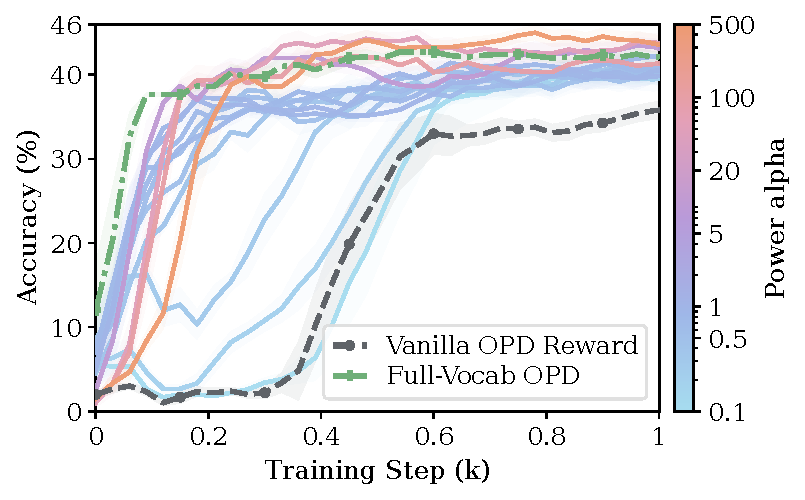
\includegraphics[width=\linewidth]{figures/fig4a_alpha_acc_s0p6b_t4b.pdf}\\[-0.5ex]
    \textbf{(a)}
  \end{minipage}\hfill
  \begin{minipage}[t]{0.245\textwidth}
    \centering
    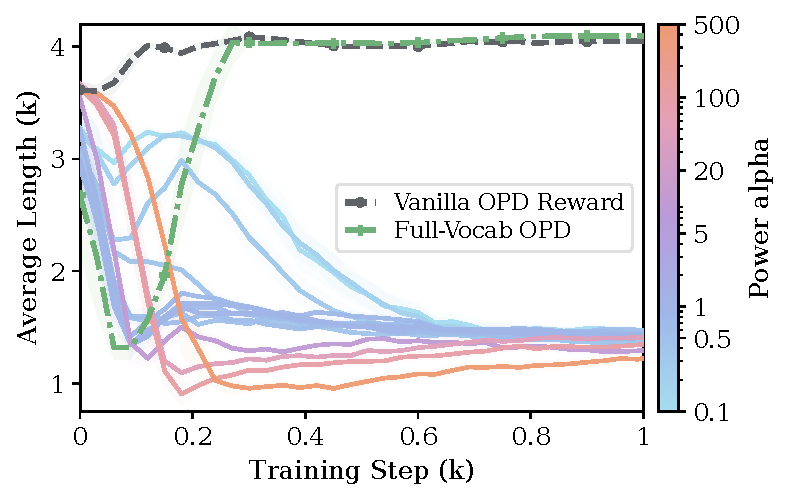
\includegraphics[width=\linewidth]{figures/fig4b_alpha_len_s0p6b_t4b.pdf}\\[-0.5ex]
    \textbf{(b)}
  \end{minipage}\hfill
  \begin{minipage}[t]{0.245\textwidth}
    \centering
    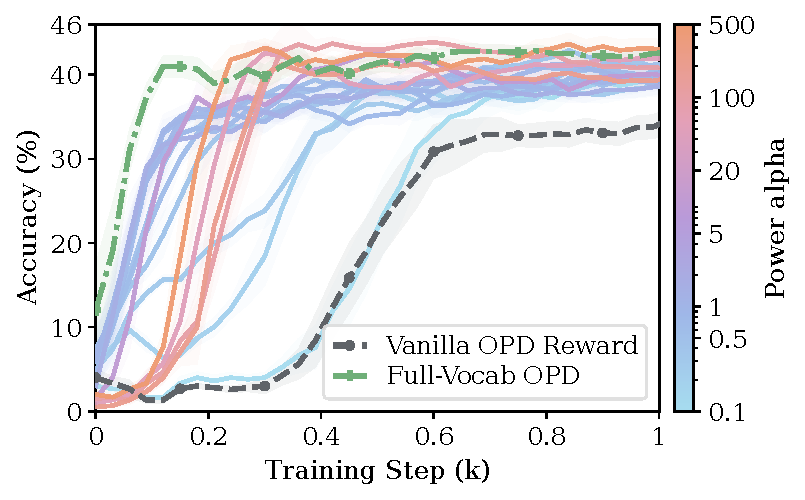
\includegraphics[width=\linewidth]{figures/fig4c_alpha_acc_s0p6b_t8b.pdf}\\[-0.5ex]
    \textbf{(c)}
  \end{minipage}\hfill
  \begin{minipage}[t]{0.245\textwidth}
    \centering
    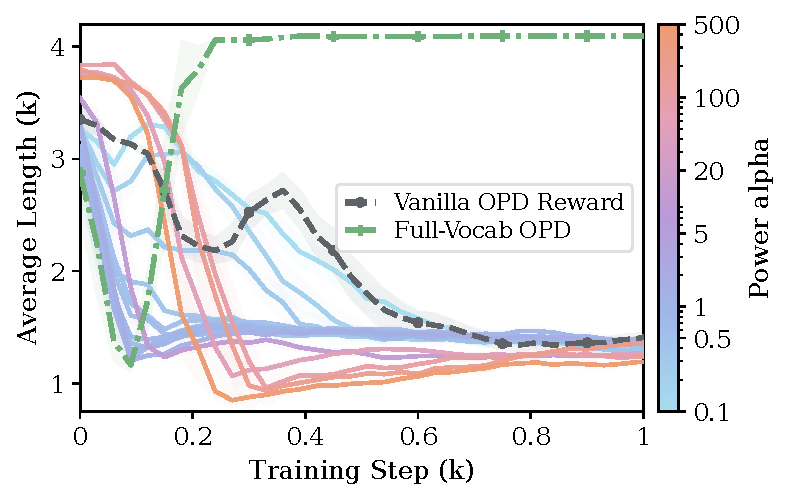
\includegraphics[width=\linewidth]{figures/fig4d_alpha_len_s0p6b_t8b.pdf}\\[-0.5ex]
    \textbf{(d)}
  \end{minipage}
  \vspace{-7pt}
    \caption{
    Training dynamics across \(\alpha\) for a Qwen3-0.6B-Base student: (a,b) accuracy and length with a Qwen3-4B teacher; (c,d) accuracy and length with a Qwen3-8B teacher.
    }
    \vspace{-10pt}
  \label{fig:alpha}
\end{figure*}

We now identify what structure a natively bounded and sign-consistent reward should take.
To obtain a tractable family, we observe that the log-ratio reward has a specific algebraic structure: it applies the same scalar transformation to each probability, then takes their difference, giving $\log\pi_T - \log\pi_\theta = h(\pi_T) - h(\pi_\theta)$ where $h(x) = \log x$.
This \emph{transform-then-subtract} class \(f_h(p,q) = h(p) - h(q)\) is attractive because sign consistency follows immediately whenever \(h\) is strictly monotone increasing: if \(p > q\), then \(h(p) > h(q)\) and \(r_t > 0\). Thus, P2 is guaranteed by construction.
The stability of the reward is then controlled entirely by the choice of $h$: the problem with the log ratio is not the transform-then-subtract structure, but the specific choice $h(x) = \log x$, which maps $[0,1]$ to $(-\infty, 0]$ and diverges at zero, making $h(\pi_T) - h(\pi_\theta)$ unbounded and violating P1.
The fix is therefore precise: keep the transform-then-subtract structure and replace $h = \log$ with a function that is both strictly monotone increasing and bounded on $[0,1]$.

\paragraph{The Box--Cox family.}
A natural and well-studied family for this purpose is the Box--Cox power transformation~\citep{boxcox1964},
\begin{equation}
  h_\alpha(x) = \frac{x^\alpha - 1}{\alpha}, \quad \alpha > 0.
  \label{eq:boxcox}
\end{equation}
For any \(\alpha>0\), \(h_\alpha\) is strictly increasing and bounded on \([0,1]\). Substituting \(h_\alpha\) into \(h(p)-h(q)\) gives \((p^\alpha-q^\alpha)/\alpha\). Since \(1/\alpha\) is a positive constant independent of tokens and policy parameters, we absorb it into the learning rate and use the rescaled reward \(p^\alpha-q^\alpha\), which is bounded in \([-1,1]\).

\paragraph{The log ratio as a limiting case.}
The standard log-ratio reward corresponds to the boundary case \(\alpha \to 0\) of the Box--Cox transformation. By the first-order Taylor expansion \(x^\alpha = 1+\alpha\log x+o(\alpha)\), we have \(h_\alpha(x)=(x^\alpha-1)/\alpha \to \log x\), and therefore \(h_\alpha(p)-h_\alpha(q)\to \log p-\log q\). However, this limit is degenerate for reward design: although each fixed \(\alpha>0\) gives a bounded transformation, its range expands as \(\alpha\to0\), recovering the unbounded log transformation and thereby violating P1.

% ============================================================
\subsection{PowerOPD}
\label{sec:poweropd}
% ============================================================

The analysis above identifies a principled family of natively bounded, sign-consistent OPD rewards. Following the policy-gradient formulation in \secref{sec:opd-as-rl}, we introduce \textbf{PowerOPD}, which uses the following stop-gradient token-level reward:
\begin{equation}
  r_t^{\alpha} = \mathrm{sg}\!\left[\pi_T(o_t \mid c_t)^{\alpha} - \pi_\theta(o_t \mid c_t)^{\alpha}\right], \quad \alpha > 0.
  \label{eq:poweropd}
\end{equation}

\paragraph{Verification.}
Since \(p,q\in[0,1]\) and \(\alpha>0\), we have \(p^\alpha,q^\alpha\in[0,1]\), so \(r_t^\alpha\in[-1,1]\): \textbf{P1 holds}.
Since \(h(x)=x^\alpha\) is strictly increasing for \(\alpha>0\), \(\pi_T>\pi_\theta \Rightarrow r_t^\alpha>0\): \textbf{P2 holds}.
Critically, both hold at the probability-to-reward mapping level, without passing through the log ratio.

\paragraph{\(\alpha\) shapes the reward sensitivity profile.}
The exponent \(\alpha\) controls how reward sensitivity is distributed across the probability range. \emph{Smaller \(\alpha\) gives relatively more sensitivity to low-probability tokens}, resembling the log ratio's emphasis on rare events while remaining bounded. \emph{Larger \(\alpha\) attenuates low-probability differences} and shifts the reward signal toward better-supported regions.